\documentclass[a4paper,12pt]{article}

\usepackage{graphicx}
\usepackage{amsmath}
\usepackage{float}

\begin{document}

\noindent
\begin{minipage}[t]{0.2\textwidth}

\includegraphics[width=2.5cm]{iiitb_logo.png}
\end{minipage}
\hfill
\begin{minipage}[t]{0.7\textwidth}
\raggedleft

{\Large \textbf{Pavithra Kune}}

COMETFWC069

\end{minipage}

\vspace{0.8cm}

\begin{center}
{\Large \textbf{GATE QUESTION Q36}}
\end{center}

\vspace{0.3cm}
\hrule
\vspace{0.5cm}

\begin{figure}[H]
\centering
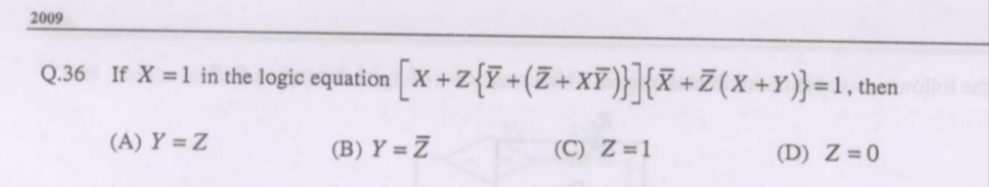
\includegraphics[width=0.8\textwidth]{question.png}
\caption{GATE Question Q36}
\end{figure}

\tableofcontents

\newpage

\section{Components}

\begin{center}
\begin{tabular}{|c|c|c|}
\hline
Component & Specification & Quantity\\
\hline
Breadboard & Standard & 1\\
Arduino Uno & ATmega328P & 1\\
IC 7474 & D Flip-Flop & 2\\
IC 7447 & BCD to 7 Segment Decoder & 1\\
Seven Segment Display & Common Anode & 1\\
Jumper Wires & Male-Male & As Required\\
\hline
\end{tabular}
\end{center}


\subsection{Breadboard}

The breadboard is used for temporary circuit connections.

\subsection{IC 7474}

The 7474 is a dual D Flip-Flop IC used to store binary data.

\subsection{IC 7447}

The 7447 is a BCD to Seven Segment Decoder Driver.

\subsection{Arduino Uno}

Arduino Uno is used to generate the clock signal and read the outputs from the 7474 ICs.

\section{Boolean Simplification}

For X=1,

[
F=\bar{Z}
]

For output 1,

[
Z=0
]

\section{Hardware Connections}

\subsection{Arduino and 7474 Connections}

\begin{center}
\begin{tabular}{|c|c|}
\hline
Arduino Pin & Function\
\hline
D13 & Clock\
D6 & W (Q1 of IC1)\
D7 & X (Q2 of IC1)\
D8 & Y (Q1 of IC2)\
D9 & Z (Q2 of IC2)\
\hline
\end{tabular}
\end{center}

\subsection{Arduino to 7447 Connections}

\begin{center}
\begin{tabular}{|c|c|}
\hline
Arduino Pin & 7447 Pin\
\hline
D2 & A\
D3 & B\
D4 & C\
D5 & D\
\hline
\end{tabular}
\end{center}

\section{Software Implementation}

\begin{verbatim}
#include <Arduino.h>

int Z;
int D,C,B,A;

void disp_7447(int D,int C,int B,int A)
{
digitalWrite(2,A);
digitalWrite(3,B);
digitalWrite(4,C);
digitalWrite(5,D);
}

void setup()
{
pinMode(2,OUTPUT);
pinMode(3,OUTPUT);
pinMode(4,OUTPUT);
pinMode(5,OUTPUT);

pinMode(6,INPUT);
pinMode(7,INPUT);
pinMode(8,INPUT);
pinMode(9,INPUT);

pinMode(13,OUTPUT);
}

void loop()
{
digitalWrite(13,HIGH);
delay(10);
digitalWrite(13,LOW);

Z = digitalRead(9);

int F = !Z;

if(F==0)
{
D=0; C=0; B=0; A=0;
}
else
{
D=0; C=0; B=0; A=1;
}

disp_7447(D,C,B,A);
delay(1000);
}
\end{verbatim}

\section{Output}

\begin{figure}[H]
\centering
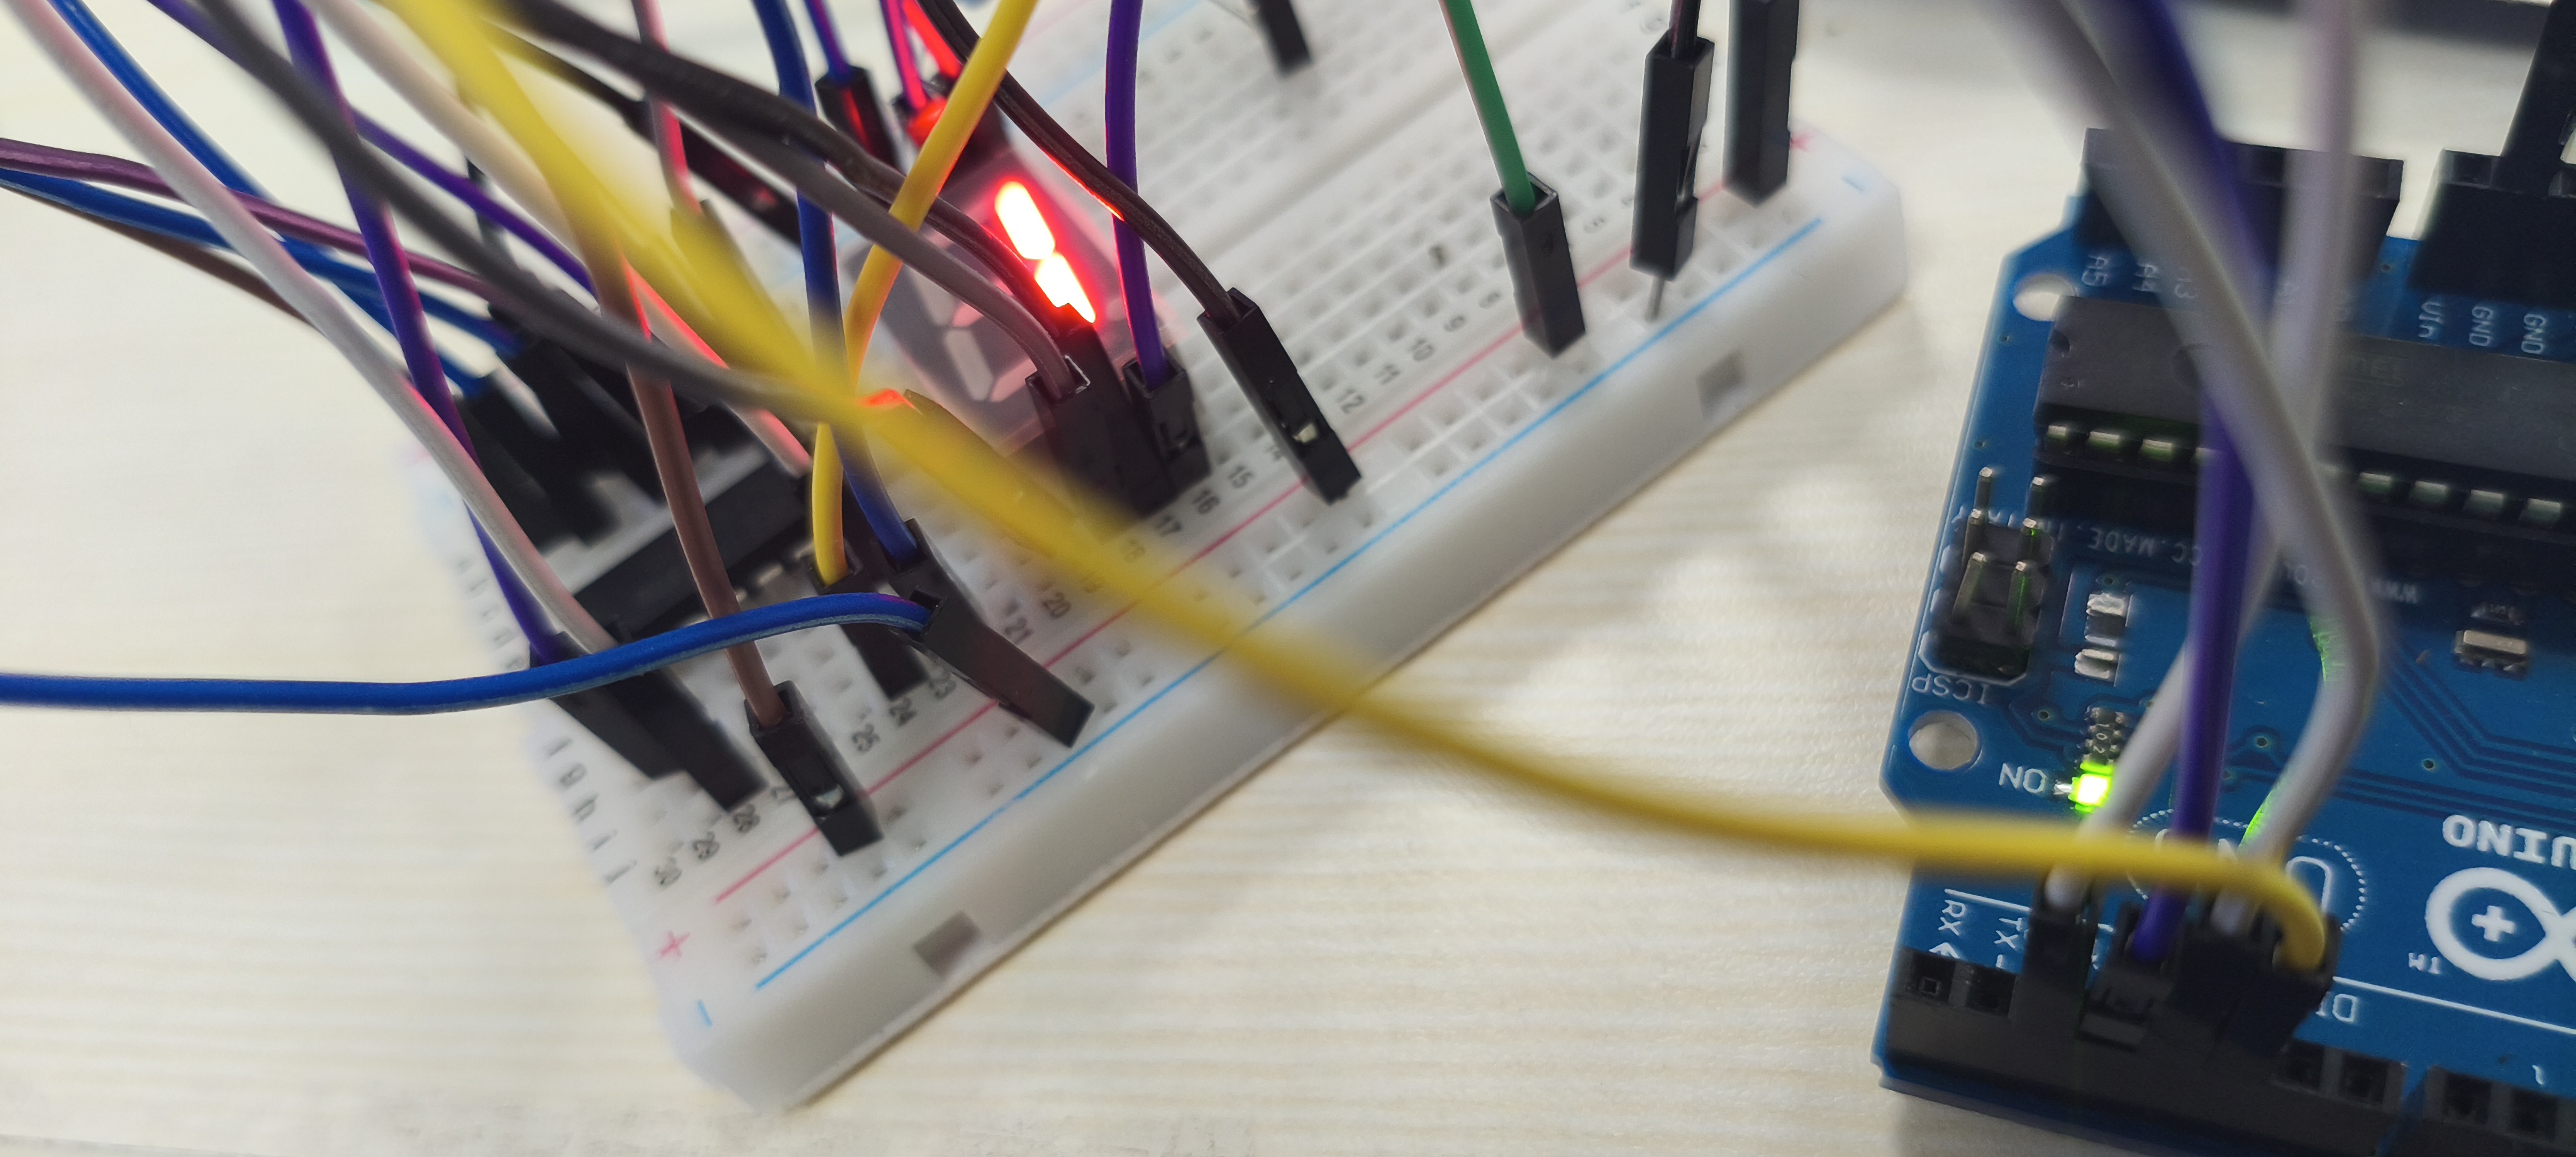
\includegraphics[width=0.45\textwidth]{output1.jpg}
\caption{Output Showing 1}
\end{figure}

\begin{figure}[H]
\centering
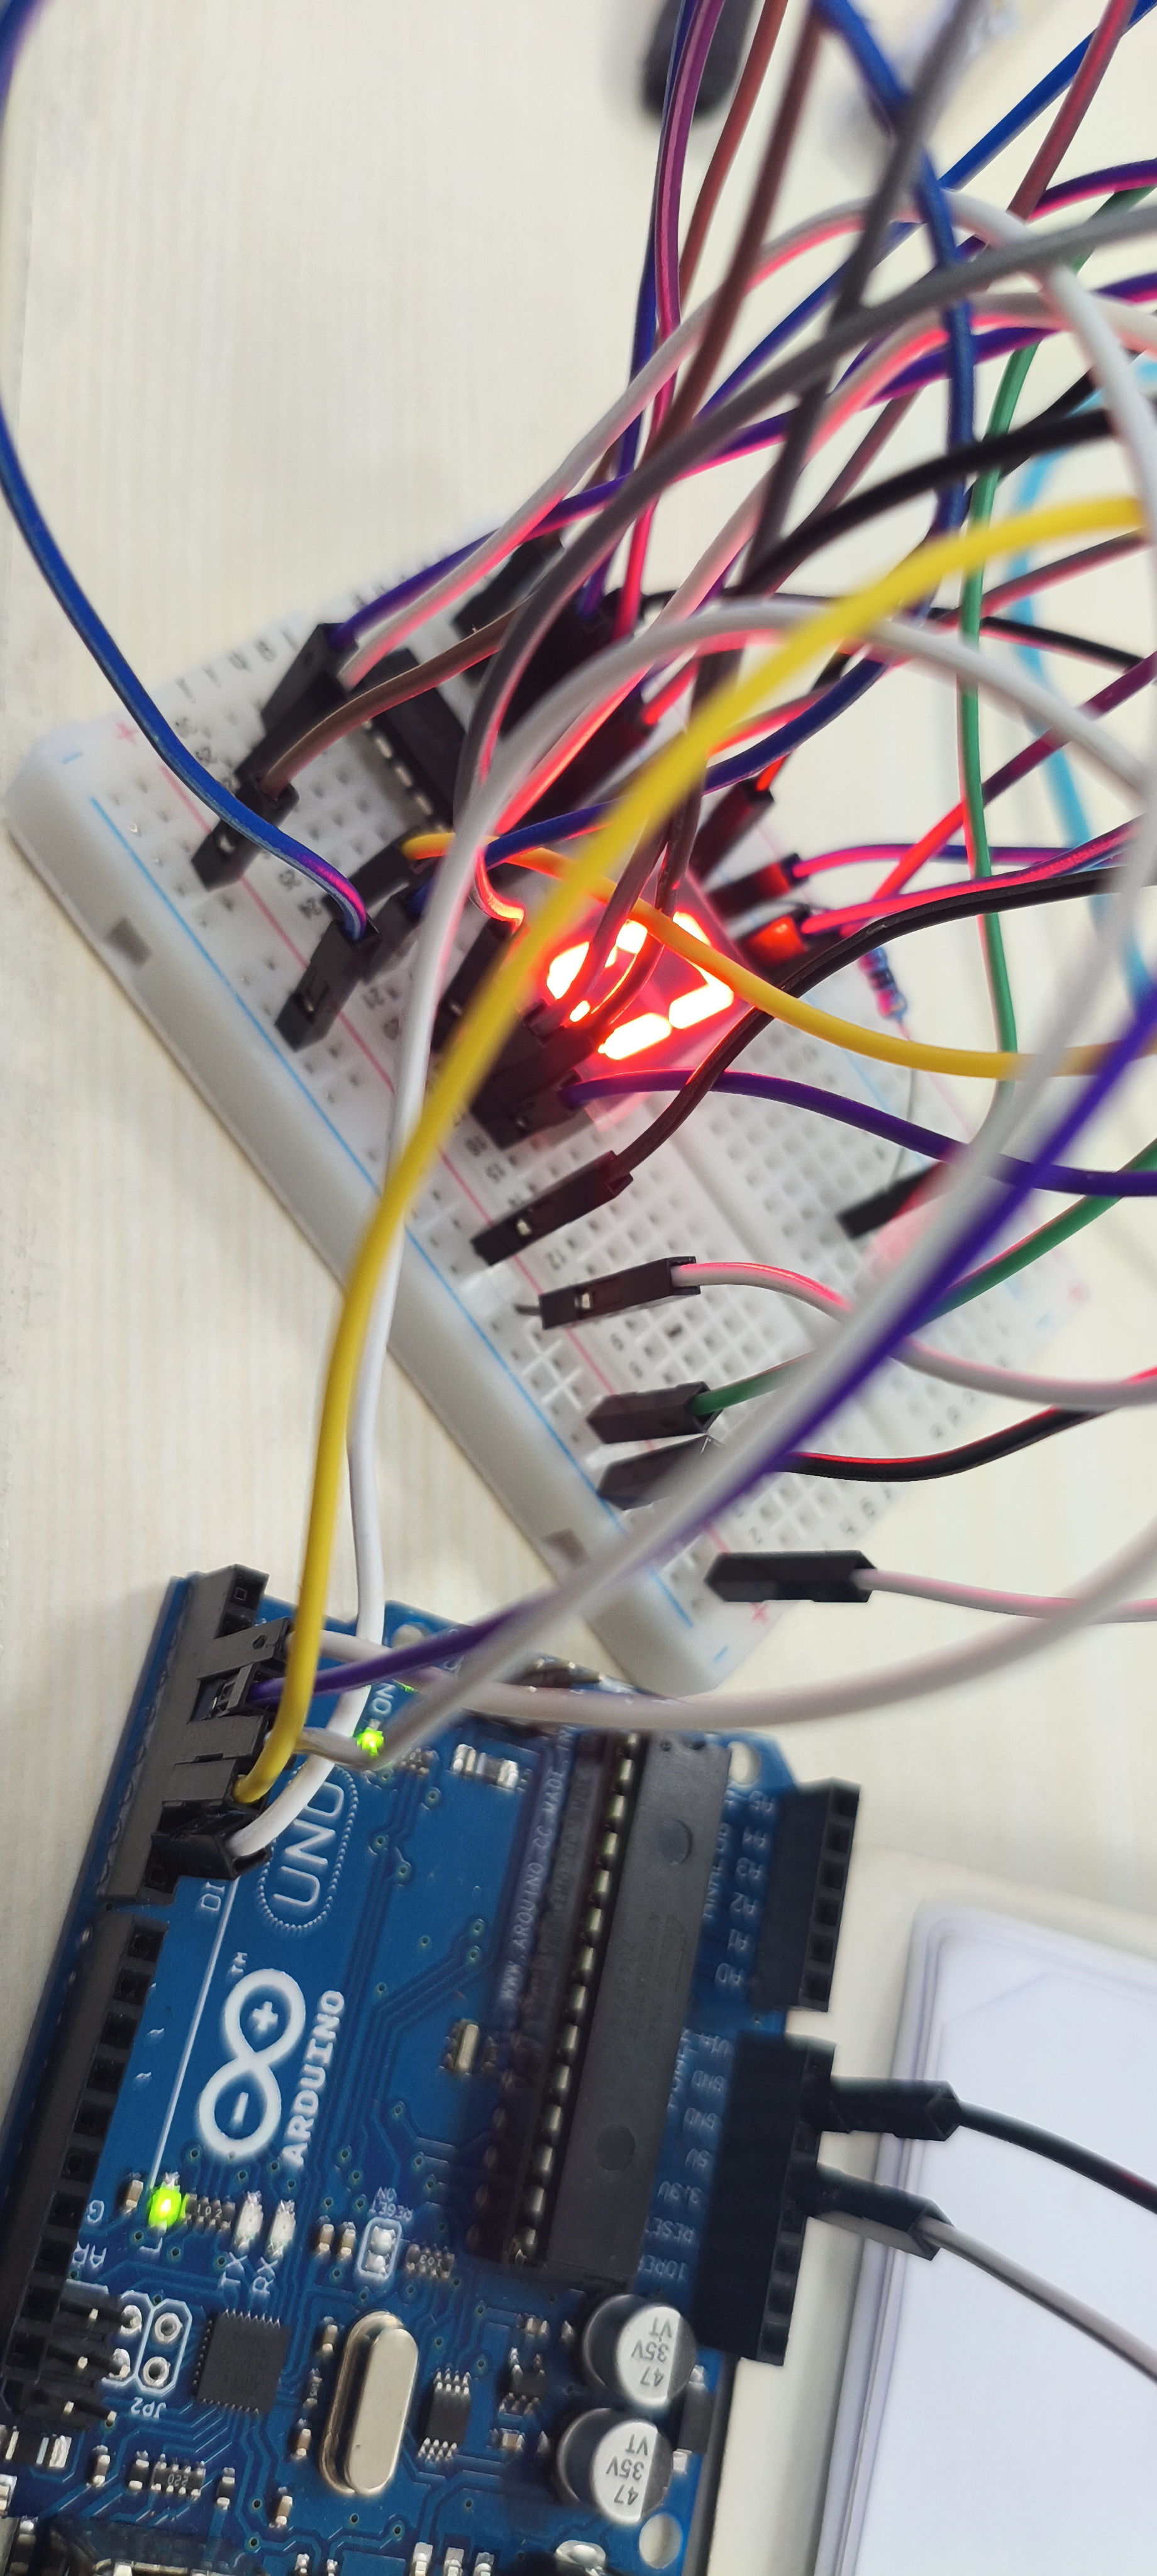
\includegraphics[width=0.45\textwidth]{output0.jpg}
\caption{Output Showing 0}
\end{figure}

\section{Result}

The given Boolean expression was implemented using 7474 D Flip-Flops, 7447 Decoder and a Seven Segment Display.

[
F=\bar{Z}
]

When Z=0,

[
F=1
]

Hence the display shows 1 on the Seven Segment Display.

\end{document}
